\documentclass[11pt,a4paper]{article}  % online-sync
% Online sync refresh: revised workshop report, 2026-08-29.

% ============================================================
% Packages
% ============================================================

\usepackage[margin=2.5cm]{geometry}
\usepackage{amsmath,amssymb,mathtools}
\usepackage{microtype}
\usepackage{tikz}
\usetikzlibrary{decorations.pathreplacing}
\usepackage{fancyhdr}
\usepackage{booktabs}
\usepackage{tabularx}
\usepackage{array}
\usepackage{graphicx}
\usepackage{float}
\usepackage{caption}
\usepackage{subcaption}
\usepackage{listings}
\usepackage{xcolor}
\usepackage[hidelinks]{hyperref}
\usepackage{algorithm}
\usepackage{algpseudocode}

\newcolumntype{Y}{>{\raggedright\arraybackslash}X}

% ============================================================
% Python code formatting
% ============================================================

\lstdefinestyle{python}{
    language=Python,
    basicstyle=\ttfamily\small,
    numbers=left,
    numberstyle=\tiny,
    frame=single,
    breaklines=true,
    columns=fullflexible,
    keepspaces=true,
    showstringspaces=false,
    tabsize=4
}

% ============================================================
% Equation numbering
% ============================================================

\newcommand{\questionequations}[1]{%
    \setcounter{equation}{0}%
    \renewcommand{\theequation}{#1.\arabic{equation}}%
    \renewcommand{\theHequation}{#1.\arabic{equation}}%
}

% ============================================================
% Student information
% ============================================================

\newcommand{\studentonename}{Ray Li}
\newcommand{\studentoneid}{1355858}

\newcommand{\studenttwoname}{James Condos}
\newcommand{\studenttwoid}{}

% ============================================================
% Header configuration
% ============================================================

\fancyhf{}
\fancyhead[L]{\textsc{ELEN90098}}
\fancyhead[R]{\textsc{Reinforcement Learning for Engineering}}

\renewcommand{\headrulewidth}{0.4pt}
\renewcommand{\footrulewidth}{0pt}

\setlength{\headheight}{14pt}

% ============================================================
% Paragraph formatting
% ============================================================

\setlength{\parindent}{0pt}
\setlength{\parskip}{0.6em}

% ============================================================
% Document
% ============================================================

\begin{document}

% ============================================================
% Cover page
% ============================================================

\hypersetup{pageanchor=false}
\begin{titlepage}
\thispagestyle{empty}
\centering

\vspace*{2.5cm}

{\Large\textsc{The University of Melbourne}\par}

\vspace{1.5cm}

{\Large ELEN90098\par}

\vspace{0.3cm}

{\Large Reinforcement Learning for Engineering\par}

\vspace{2.5cm}

{\Huge\bfseries Workshop 1\par}

\vspace{0.4cm}

{\LARGE Multi-Armed Bandits\par}

\vfill

\begin{tabular}{rl}
    \textbf{Student 1:}     & \studentonename \\[0.15cm]
    \textbf{Student ID:}   & \studentoneid \\[0.6cm]

    \textbf{Student 2:}     & \studenttwoname \\[0.15cm]
    \textbf{Student ID:}   & \studenttwoid
\end{tabular}

\vfill

{\large Semester 2, 2026\par}

\vspace{1.5cm}

\end{titlepage}
\hypersetup{pageanchor=true}

% ============================================================
% Main document
% ============================================================

\pagestyle{fancy}
\setcounter{page}{1}

% ------------------------------------------------------------
% Question 1
% ------------------------------------------------------------

\section*{Question 1}
\questionequations{1}
Let $\mathcal{A}$ denote the set of available arms. At time step $k$, the
algorithm selects an arm $A_k\in\mathcal{A}$ and receives a random reward
$R_k$. The true action value of arm $a$ is
\[
    q^\ast(a)
    =
    \mathbb{E}\!\left[R_k \mid A_k=a\right],
\]
which is the expected reward obtained when arm $a$ is selected.

Let
\[
    a^\ast \in \arg\max_{a\in\mathcal{A}} q^\ast(a)
\]
be an optimal arm. The best achievable expected reward per time step is then
\[
    R^\ast
    =
    q^\ast(a^\ast)
    =
    \max_{a\in\mathcal{A}} q^\ast(a).
\]
Thus, $R^\ast$ is a deterministic expected reward, whereas $R_k$ is the
random reward actually observed at time step $k$.

The cumulative expected regret after $t$ time steps is defined as
\begin{equation}
    \operatorname{Regret}_t
    =
    \mathbb{E}\!\left[
        \sum_{k=1}^{t}
        \left(R^\ast-R_k\right)
    \right].
    \label{eq:q1-regret}
\end{equation}
The expectation in \eqref{eq:q1-regret} accounts for the randomness in the
observed rewards and, where applicable, the randomisation of the bandit
policy. In particular, if arm $a$ is selected at time $k$, its expected
one-step regret is
\[
    R^\ast-q^\ast(a)\geq 0.
\]
Hence, regret measures the expected cumulative loss in reward caused by not
knowing the optimal arm in advance.

A bandit algorithm is said to have \emph{sublinear regret} if
\begin{equation}
    \lim_{t\to\infty}
    \frac{\operatorname{Regret}_t}{t}
    =
    0,
    \label{eq:q1-sublinear-regret}
\end{equation}
or equivalently,
\[
    \operatorname{Regret}_t=o(t).
\]

Using \eqref{eq:q1-regret},
\begin{align}
    \frac{\operatorname{Regret}_t}{t}
    &=
    \frac{1}{t}
    \mathbb{E}\!\left[
        \sum_{k=1}^{t}
        \left(R^\ast-R_k\right)
    \right]
    \notag\\
    &=
    R^\ast
    -
    \mathbb{E}\!\left[
        \frac{1}{t}\sum_{k=1}^{t}R_k
    \right].
    \label{eq:q1-average-regret}
\end{align}
Therefore, by \eqref{eq:q1-sublinear-regret} and
\eqref{eq:q1-average-regret}, sublinear regret implies
\[
    \lim_{t\to\infty}
    \mathbb{E}\!\left[
        \frac{1}{t}\sum_{k=1}^{t}R_k
    \right]
    =
    R^\ast.
\]

Thus, the significance of sublinear regret is that the average expected
reward of the learning algorithm converges to the best achievable expected
reward. Although the algorithm incurs regret while exploring and learning
which arm is optimal, the regret per time step vanishes asymptotically.

\newpage

% ------------------------------------------------------------
% Question 2
% ------------------------------------------------------------

\section*{Question 2}
\questionequations{2}
% Online sync refresh: revised workshop report, 2026-08-29.
The definition of sublinear regret requires
\[
    \lim_{T\to\infty}
    \frac{\operatorname{Regret}_T}{T}
    =
    0,
\]
which is the standard asymptotic criterion used in multi-armed bandit
regret analysis. Therefore, a natural numerical
test is to estimate the regret at a sequence of increasingly large horizons
and examine its asymptotic growth.

Suppose the experiment is repeated independently for $M$ runs, and let
$A_t^{(r)}$ denote the arm selected at time $t$ in run $r$. Since the
synthetic bandit environment is known to us, the optimal expected reward is
\[
    R^\ast
    =
    \max_{a\in\mathcal A} q^\ast(a).
\]
The true action values $q^\ast(a)$ are used only for performance evaluation
after an action has been selected; they are not made available to the
learning algorithm.

For run $r$, define the cumulative pseudo-regret at horizon $T$ as
\[
    C_T^{(r)}
    =
    \sum_{t=1}^{T}
    \left[
        R^\ast-q^\ast\!\left(A_t^{(r)}\right)
    \right].
\]
Averaging over the $M$ independent reruns gives the empirical estimate
\[
    \widehat{\operatorname{Regret}}_T
    =
    \frac{1}{M}
    \sum_{r=1}^{M}
    C_T^{(r)}.
\]

The first diagnostic is the normalised empirical regret
\begin{equation}
    \widehat{\rho}_T
    =
    \frac{\widehat{\operatorname{Regret}}_T}{T}.
    \label{eq:q2-normalised-regret}
\end{equation}
By the definition of sublinear regret,
\eqref{eq:q2-normalised-regret} should approach zero as $T$ increases.
However, examining this quantity at only one finite horizon can be
misleading. For example, if
\[
    \operatorname{Regret}_T=C+cT,
    \qquad c>0,
\]
then
\[
    \frac{\operatorname{Regret}_T}{T}
    =
    \frac{C}{T}+c
\]
may decrease substantially with $T$, even though it eventually converges
to the positive constant $c$ and the regret is therefore linear.

To distinguish such transient behaviour from genuinely sublinear growth,
we additionally evaluate the incremental regret rate between successive
horizons $T_i<T_{i+1}$:
\begin{equation}
    \widehat{s}_i
    =
    \frac{
        \widehat{\operatorname{Regret}}_{T_{i+1}}
        -
        \widehat{\operatorname{Regret}}_{T_i}
    }{
        T_{i+1}-T_i
    }.
    \label{eq:q2-incremental-rate}
\end{equation}
This is the average slope of the cumulative-regret curve over the interval
$[T_i,T_{i+1}]$.

The use of \eqref{eq:q2-incremental-rate} follows directly from the
definition of sublinear regret. Consider geometrically increasing horizons
$T_{i+1}=cT_i$, where $c>1$. Since cumulative pseudo-regret is non-negative
and non-decreasing,
\[
    0
    \leq
    \widehat{s}_i
    \leq
    \frac{
        \widehat{\operatorname{Regret}}_{cT_i}
    }{
        (c-1)T_i
    }
    =
    \frac{c}{c-1}
    \frac{
        \widehat{\operatorname{Regret}}_{cT_i}
    }{
        cT_i
    }.
\]
Hence, if the underlying regret is sublinear, the right-hand side approaches
zero as the horizon increases, and therefore the incremental regret rate
should also approach zero. In contrast, if
\[
    \operatorname{Regret}_T
    \sim c_0 T,
    \qquad c_0>0,
\]
then
\[
    \widehat{s}_i
    \longrightarrow
    c_0,
\]
so a positive late-horizon plateau in the incremental regret rate provides
numerical evidence of linear regret.

As a supplementary diagnostic, the local effective growth exponent is
estimated by
\[
    \widehat{\alpha}_i
    =
    \frac{
        \log
        \widehat{\operatorname{Regret}}_{T_{i+1}}
        -
        \log
        \widehat{\operatorname{Regret}}_{T_i}
    }{
        \log T_{i+1}-\log T_i
    }.
\]
If locally
$\widehat{\operatorname{Regret}}_T\approx CT^\alpha$, then
$\widehat{\alpha}_i\approx\alpha$. Thus,
$\widehat{\alpha}_i$ approaching $1$ supports locally approximately linear
power-law growth, whereas values remaining below $1$ support a sublinear
power-law interpretation. However, $\widehat{\alpha}_i$ is neither a
necessary nor a sufficient test for sublinear regret. For example, the
sublinear function $T/\log T$ also has a local effective exponent approaching
$1$. The normalised regret and incremental regret rate are therefore the
primary diagnostics, while the effective exponent is supplementary.

The proposed numerical procedure is therefore to simulate each algorithm
up to a maximum horizon and record its cumulative pseudo-regret at several
geometrically increasing horizons, for example
\[
    T\in
    \{10^3,\,3\times10^3,\,10^4,\,3\times10^4,\,10^5\}.
\]
The experiment is repeated for many independent runs and
$\widehat{\operatorname{Regret}}_T$,
$\widehat{\rho}_T$,
$\widehat{s}_i$, and
$\widehat{\alpha}_i$
are calculated.

Numerical behaviour is considered consistent with sublinear regret when,
over the largest simulated horizons,
\[
    \widehat{\rho}_T
    \longrightarrow 0
    \qquad\text{and}\qquad
    \widehat{s}_i
    \longrightarrow 0,
\]
based on their observed multi-horizon trends. Conversely, a positive
late-horizon incremental regret rate provides evidence of a linear
component. The effective exponent may support a local power-law
interpretation, but it is not used as an automatic classification rule.

Because only finitely many horizons and reruns can be simulated, this test
cannot prove an asymptotic regret property. It provides numerical evidence
by examining whether the observed large-horizon growth is consistent with
the mathematical definition of sublinear regret.


The proposed numerical procedure is summarised in
Algorithm~\ref{alg:q2-sublinear-test}.

\begin{algorithm}[H]
\caption{Multi-horizon numerical test for sublinear regret}
\label{alg:q2-sublinear-test}
\begin{algorithmic}[1]
\Require Bandit policy $\pi$, horizons
$T_1<\cdots<T_L$, number of reruns $M$

\For{$r=1,\ldots,M$}
    \State Simulate $\pi$ up to $T_L$
    \State Record cumulative pseudo-regret
    $C_{T_i}^{(r)}$ at each horizon $T_i$
\EndFor

\For{$i=1,\ldots,L$}
    \State Estimate
    $\widehat{\operatorname{Regret}}_{T_i}
    \gets \frac{1}{M}\sum_{r=1}^{M}C_{T_i}^{(r)}$
    \State Compute
    $\widehat{\rho}_{T_i}
    \gets \widehat{\operatorname{Regret}}_{T_i}/T_i$
\EndFor

\For{$i=1,\ldots,L-1$}
    \State Compute incremental regret rate
    \[
        \widehat{s}_i
        \gets
        \frac{
            \widehat{\operatorname{Regret}}_{T_{i+1}}
            -
            \widehat{\operatorname{Regret}}_{T_i}
        }{
            T_{i+1}-T_i
        }
    \]
    \State Compute effective exponent
    \[
        \widehat{\alpha}_i
        \gets
        \frac{
            \log \widehat{\operatorname{Regret}}_{T_{i+1}}
            -
            \log \widehat{\operatorname{Regret}}_{T_i}
        }{
            \log T_{i+1}-\log T_i
        }
    \]
\EndFor

\State Examine the late-horizon trends of the primary diagnostics
$\widehat{\rho}_{T_i}$ and $\widehat{s}_i$

\State Use $\widehat{\alpha}_i$ only as a supplementary local
power-law diagnostic

\State Interpret the measured trends manually; do not apply a fixed
numerical classification threshold

\end{algorithmic}
\end{algorithm}


\newpage

% ------------------------------------------------------------
% Question 3
% ------------------------------------------------------------

\section*{Question 3}
\questionequations{3}
% Online sync refresh: revised workshop report, 2026-08-29. figure-path-fix
The supplied $\epsilon$-greedy implementation was extended using the
multi-horizon numerical procedure proposed in
Algorithm~\ref{alg:q2-sublinear-test}. For each selected action $A_t$,
the instantaneous pseudo-regret was evaluated as
\[
    R^\ast-q^\ast(A_t),
\]
where $q^\ast$ was used only for post-action performance evaluation and was
not available to the learning algorithm.

The six exploration schedules considered were
\[
\begin{aligned}
    &\epsilon_t=0, \qquad
    \epsilon_t=0.01, \qquad
    \epsilon_t=0.10,\\
    &\epsilon_t=
    \min\left\{
        \left(
            \frac{k\log(t+1)}{t+1}
        \right)^{1/3},
        1
    \right\},\\
    &\epsilon_t=0.99^t, \qquad
    \epsilon_t=0.90^t.
\end{aligned}
\]
The $t+1$ form in the polynomial schedule accounts for Python's zero-based
indexing. The final exponential-decay case in the supplied code was also
corrected to use $0.90^t$, consistent with its stated label.

To reduce the risk of mistaking finite-horizon transient behaviour for an
asymptotic trend, each policy was simulated for $M=500$ independent reruns
up to
\[
    T_{\max}=10^5,
\]
with cumulative pseudo-regret recorded at
\[
    T_i\in
    \{10^3,\,3\times10^3,\,10^4,\,3\times10^4,\,10^5\}.
\]
At these horizons, the normalised regret $\widehat{\rho}_{T_i}$,
incremental regret rate $\widehat{s}_i$, and effective regret exponent
$\widehat{\alpha}_i$ defined in Question~2 were evaluated. The first two are
the primary definition-based diagnostics. The effective exponent is a
supplementary local log-log slope and is not used as a necessary or
sufficient test for sublinear regret.

\begin{figure}[H]
    \centering
    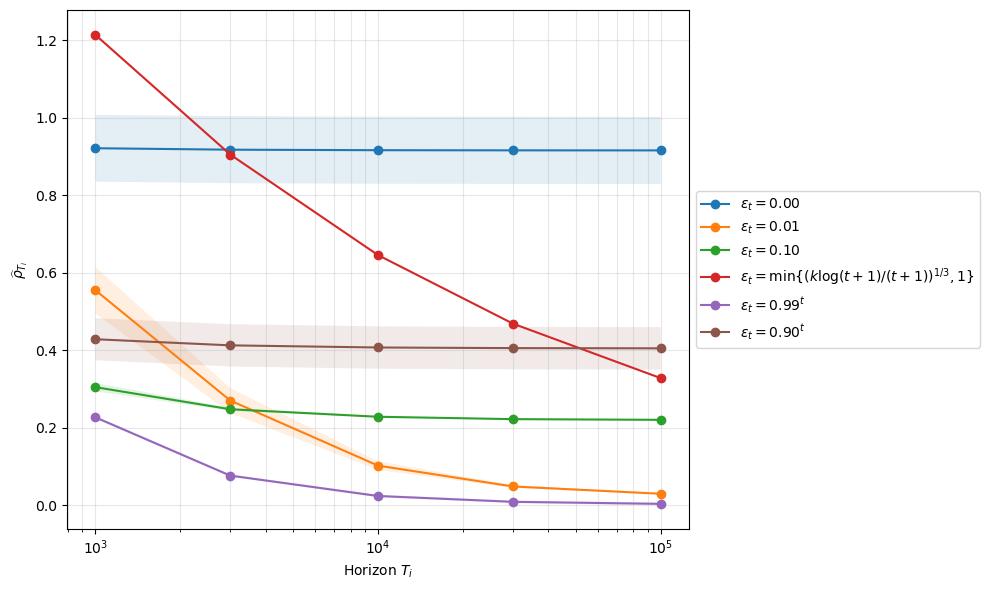
\includegraphics[width=0.92\linewidth]
    {figures/epsilon_multihorizon_normalised_regret.png}
    \caption{Normalised empirical cumulative pseudo-regret
    $\widehat{\rho}_{T_i}$ for the six $\epsilon$-greedy schedules.
    Shaded regions represent approximate 95\% Monte Carlo confidence
    intervals.}
    \label{fig:q3-normalised-regret}
\end{figure}

Figure~\ref{fig:q3-normalised-regret} provides the diagnostic most directly
related to the definition of sublinear regret. The curves for
$\epsilon_t=0$, $\epsilon_t=0.10$, and $\epsilon_t=0.90^t$ clearly approach
positive values and are therefore inconsistent with
$\widehat{\rho}_{T_i}\to0$. The cases $\epsilon_t=0.01$ and
$\epsilon_t=0.99^t$ are less obvious from normalised regret alone because
their curves continue decreasing over the simulated horizons. This motivates
the additional diagnostics introduced in Question~2.

\begin{figure}[H]
    \centering
    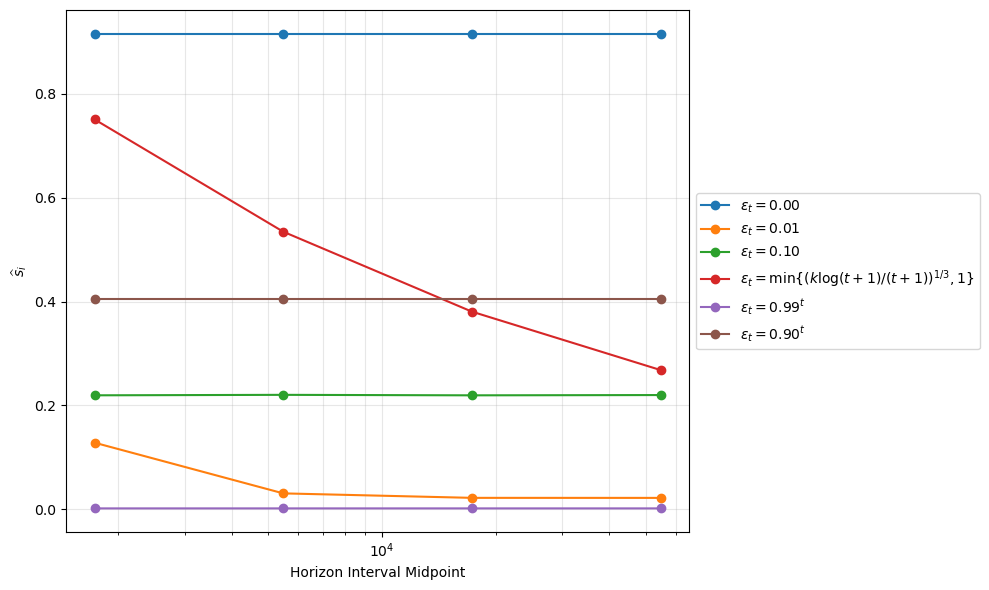
\includegraphics[width=0.92\linewidth]
    {figures/epsilon_incremental_regret_rate.png}
    \caption{Incremental regret rate $\widehat{s}_i$ between consecutive
    simulation horizons.}
    \label{fig:q3-incremental-regret}
\end{figure}

Figure~\ref{fig:q3-incremental-regret} shows whether additional regret is
still accumulating at a non-zero rate. For a linear-regret policy,
$\widehat{s}_i$ should approach a positive constant, whereas for sublinear
regret it should decrease towards zero. The polynomial schedule is the only
case exhibiting persistent decay over all four intervals:
\[
    0.7507
    \;\to\;
    0.5345
    \;\to\;
    0.3805
    \;\to\;
    0.2681.
\]
In contrast, the other schedules eventually exhibit an approximately
constant positive mean incremental regret rate. For $\epsilon_t=0.99^t$,
the corresponding run-level slopes must also be inspected because the mean
is produced by a rare-event mixture.

\begin{figure}[H]
    \centering
    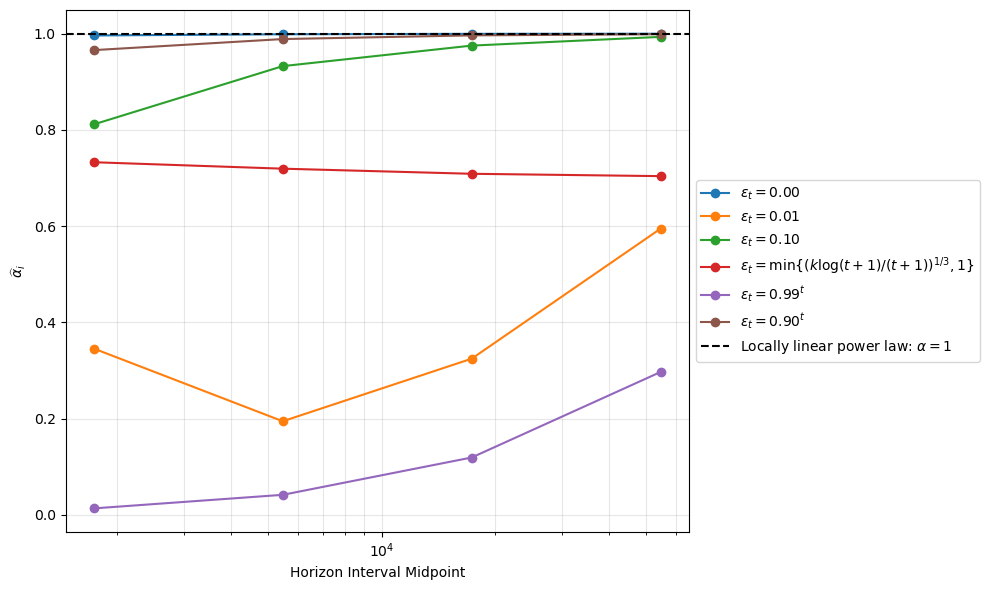
\includegraphics[width=0.92\linewidth]
    {figures/epsilon_effective_regret_exponent.png}
    \caption{Effective regret exponent $\widehat{\alpha}_i$ between
    consecutive horizons. The dashed line $\alpha=1$ corresponds to
    linear power-law growth.}
    \label{fig:q3-effective-exponent}
\end{figure}

The effective exponents in Figure~\ref{fig:q3-effective-exponent} provide a
supplementary indication of the growth order. In particular,
$\widehat{\alpha}_i$ approaches one for several of the policies exhibiting
linear regret, whereas the polynomial schedule remains well below one,
decreasing from approximately $0.733$ to $0.704$. An exponent approaching
one does not by itself prove linear regret: for example, the sublinear
function $T/\log T$ also has a local effective exponent approaching one.

The complete multi-horizon diagnostics are summarised in
Table~\ref{tab:q3-diagnostics}.

\begin{table}[H]
\centering
\caption{Measured multi-horizon numerical diagnostics for the six
$\epsilon$-greedy schedules. Interpretations are given separately in the
text.}
\label{tab:q3-diagnostics}
\resizebox{\textwidth}{!}{
\begin{tabular}{lccc}
\toprule
\textbf{Schedule}
& $\widehat{\rho}_{10^5}$
& $\widehat{s}_1\rightarrow\widehat{s}_4$
& $\widehat{\alpha}_1\rightarrow\widehat{\alpha}_4$ \\
\midrule

$\epsilon_t=0$
& $0.9158$
& $0.9157\to0.9157\to0.9157\to0.9157$
& $0.9963\to0.9988\to0.9996\to0.9999$ \\

$\epsilon_t=0.01$
& $0.0300$
& $0.1282\to0.0306\to0.0220\to0.0219$
& $0.3456\to0.1946\to0.3246\to0.5948$ \\

$\epsilon_t=0.10$
& $0.2207$
& $0.2194\to0.2203\to0.2194\to0.2200$
& $0.8115\to0.9326\to0.9752\to0.9934$ \\

Polynomial decay
& $0.3283$
& $0.7507\to0.5345\to0.3805\to0.2681$
& $0.7329\to0.7195\to0.7089\to0.7040$ \\

$\epsilon_t=0.99^t$
& $0.0040$
& $0.001699\to0.001697\to0.001697\to0.001697$
& $0.0135\to0.0417\to0.1193\to0.2970$ \\

$\epsilon_t=0.90^t$
& $0.4052$
& $0.4049\to0.4049\to0.4049\to0.4049$
& $0.9658\to0.9888\to0.9965\to0.9989$ \\

\bottomrule
\end{tabular}}
\end{table}

Table~\ref{tab:q3-diagnostics} contains measured quantities only. The
following conclusions are manual interpretations of the diagnostic trends,
not outputs of a threshold-based classifier.

For $\epsilon_t=0$, no systematic exploration occurs. The algorithm may
therefore commit permanently to a suboptimal arm. Its incremental regret
rate remains at approximately $0.916$, while
$\widehat{\alpha}_i\to1$, providing clear evidence of linear regret.

For the fixed exploration rate $\epsilon_t=0.10$,
$\widehat{s}_i$ remains almost exactly constant at approximately $0.22$ and
$\widehat{\alpha}_i$ approaches one. Hence, its cumulative regret is clearly
linear. The case $\epsilon_t=0.01$ illustrates why the incremental-rate
diagnostic is useful: although its normalised regret is still decreasing at
$T=10^5$, its incremental regret rate settles at approximately $0.0219$.
Thus the observed behaviour is consistent with a regret curve of the form
\[
    \operatorname{Regret}_T
    \approx
    C+cT,
    \qquad c>0,
\]
where the transient term $C/T$ causes the normalised regret to continue
decreasing before eventually approaching the positive constant $c$.

The polynomial schedule
\[
    \epsilon_t=
    \min\left\{
        \left(
            \frac{k\log(t+1)}{t+1}
        \right)^{1/3},
        1
    \right\}
\]
is the only case that is numerically consistent with sublinear regret.
Its normalised regret continues to decrease, its incremental regret rate
decreases persistently towards zero, and its effective exponent remains
well below one across the largest simulated horizons.

For $\epsilon_t=0.90^t$, exploration decays so rapidly that the algorithm can
become permanently committed to a suboptimal arm. Correspondingly,
$\widehat{s}_i$ approaches the positive value $0.4049$ and
$\widehat{\alpha}_i\to1$, indicating linear regret.

The slower exponential schedule $\epsilon_t=0.99^t$ performs substantially
better at finite horizons, but the multi-horizon test reveals behaviour that
was not apparent in the shorter experiment. Over the final interval
$[30000,100000]$, $499$ of the $500$ reruns have essentially zero individual
late slope, while one rerun has a positive slope of approximately $0.848290$.
Consequently, the mean late slope is
\[
    \widehat{s}_i\approx0.001697,
\]
but this value is a rare-event mixture rather than a precisely estimated
population coefficient. Its effective exponent increases from approximately
$0.014$ to $0.297$ as the horizon grows. Together with the fact that
$\sum_t 0.99^t<\infty$, so exploration can cease before a run identifies the
optimal arm, the result is consistent with a possible linear-regret
component rather than reliable sublinear convergence.

Therefore, among the six tested exploration schedules, the only policy
numerically consistent with sublinear regret is
\[
    \epsilon_t=
    \min\left\{
        \left(
            \frac{k\log(t+1)}{t+1}
        \right)^{1/3},
        1
    \right\}.
\]
The numerical conclusion agrees with the theoretical result that exploration
must decay sufficiently slowly to maintain learning while its long-run
frequency approaches zero. Since only finite horizons and finitely many
reruns are simulated, these results provide numerical evidence of the
asymptotic growth regime rather than a mathematical proof.


\newpage

% ------------------------------------------------------------
% Question 4
% ------------------------------------------------------------

\section*{Question 4}
\questionequations{4}
% Online sync refresh: revised workshop report, 2026-08-29. figure-path-fix
To investigate whether UCB learns the true value of each arm, the algorithm
was simulated for \(T=10^4\) steps over \(M=300\) independent reruns for
\(c\in\{0,1,2\}\). Each arm was selected once initially to avoid an undefined
confidence bonus. Thereafter, actions were selected using the UCB rule and
the empirical action-value estimate \(Q_t(a)\) was updated by the sample
average.

Since the true values \(q^\ast(a)\) are known in the simulated environment,
the estimation accuracy of each arm was measured using
\[
    \operatorname{RMSE}_t(a)
    =
    \sqrt{
        \frac{1}{M}
        \sum_{r=1}^{M}
        \left(
            Q_t^{(r)}(a)-q^\ast(a)
        \right)^2
    }.
\]
A decreasing RMSE therefore indicates that the empirical estimate of an arm
is approaching its true value.

\begin{figure}[H]
    \centering
    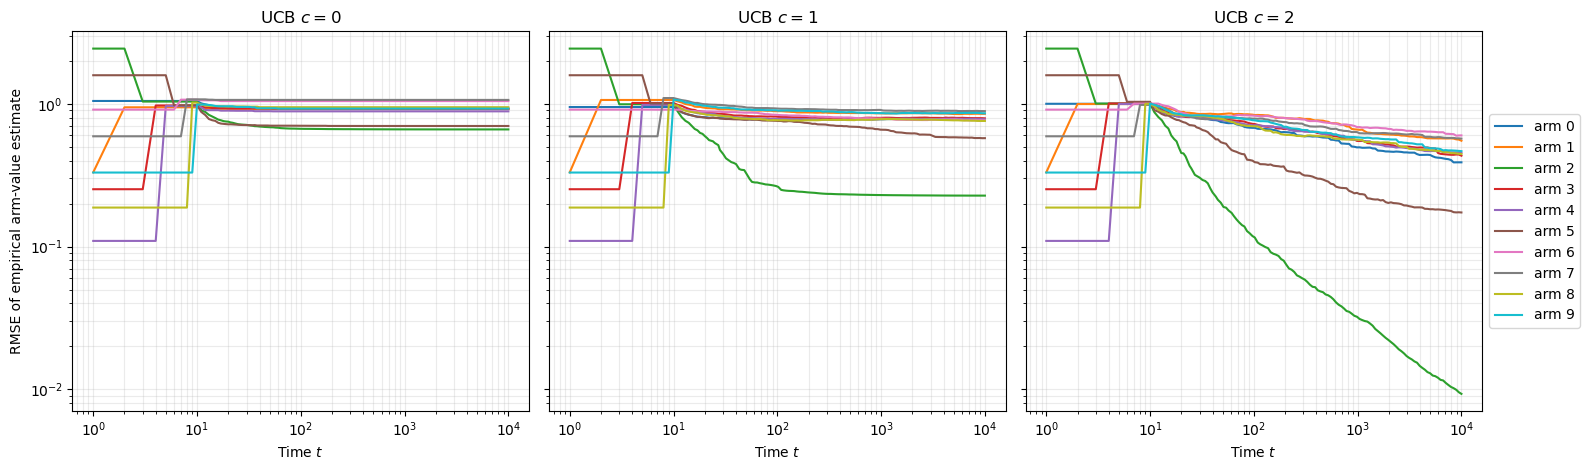
\includegraphics[width=\linewidth]
    {figures/q4_ucb_arm_value_rmse.png}
    \caption{RMSE of the empirical value estimate for each arm under UCB
    with \(c=0,1,2\), averaged over \(300\) independent reruns.}
    \label{fig:q4-ucb-rmse}
\end{figure}

As shown in Figure~\ref{fig:q4-ucb-rmse}, the amount of exploration has a
strong effect on value estimation. For \(c=0\), the confidence bonus
vanishes and the algorithm becomes purely greedy after the initial pulls.
Consequently, many arms are never revisited and their estimation errors do
not decrease. The final mean arm-wise RMSE is approximately \(0.898\).

For \(c=1\), UCB continues to revisit uncertain arms, reducing the final mean
arm-wise RMSE to approximately \(0.725\). However, highly suboptimal arms
are sampled only a few times by \(T=10^4\), so their estimates remain noisy.
Increasing the exploration coefficient to \(c=2\) produces substantially more
accurate estimates across the arms, reducing the final mean arm-wise RMSE to
approximately \(0.409\).

At the finite horizon $T=10^4$, $c=2$ therefore gives substantially better
arm-value estimation, while $c=1$ still leaves several poor arms sparsely
sampled and has not accurately learned every arm. Asymptotically, if an
arm's count remained bounded while time increased, its bonus
$c\sqrt{\log(t+1)/N_t(a)}$ would diverge and force that arm to be revisited.
Thus exploratory UCB supports eventual learning of every arm, but the
numerical results show that this can be extremely slow for highly
suboptimal arms. The degenerate case $c=0$ does not in general learn every
arm because it ceases systematic exploration.


\newpage

% ------------------------------------------------------------
% Question 5
% ------------------------------------------------------------

\section*{Question 5}
\questionequations{5}
% Online sync refresh: revised workshop report, 2026-08-29. figure-path-fix
The UCB and $\epsilon$-greedy algorithms were compared on the same
10-armed bandit over a horizon of $T=10^4$, with the experiment repeated
over $M=300$ independent reruns. For each run, cumulative pseudo-regret was
computed as
\[
    \sum_{t=1}^{T}
    \left[
        R^\ast-q^\ast(A_t)
    \right],
\]
and then averaged across reruns. The comparison includes UCB with
$c\in\{0,1,2\}$ and the six $\epsilon$-greedy schedules considered
previously.

\begin{figure}[H]
    \centering
    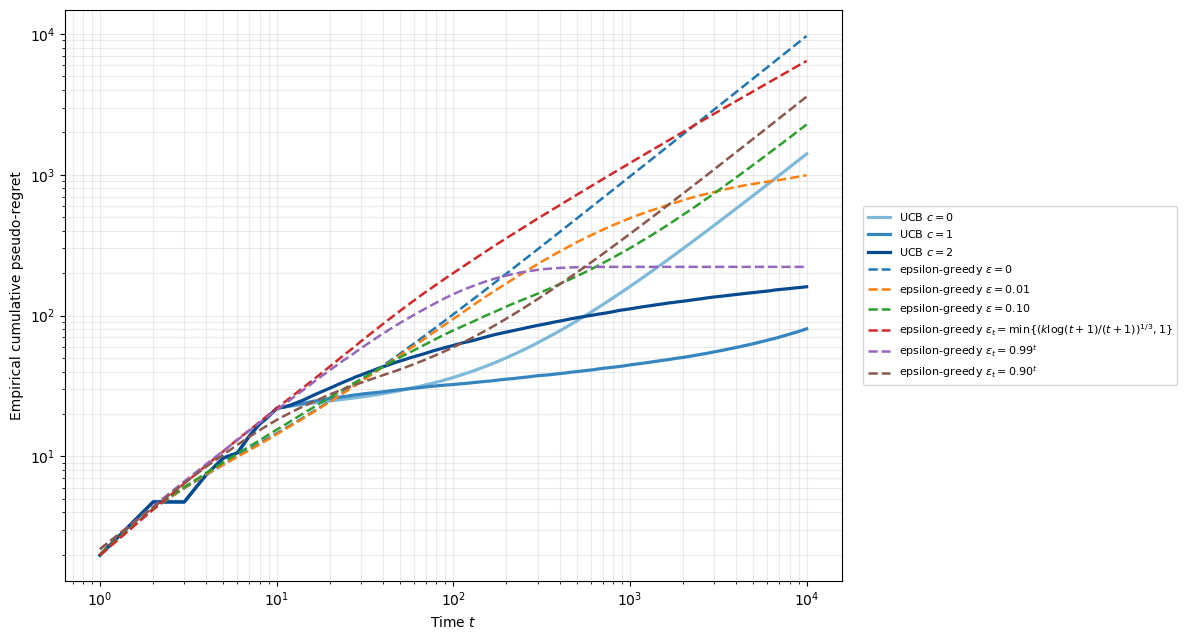
\includegraphics[width=0.82\linewidth]
    {figures/q5_ucb_vs_epsilon_regret.png}
    \caption{Empirical cumulative pseudo-regret of UCB and
    $\epsilon$-greedy algorithms over $T=10^4$ time steps.}
    \label{fig:q5-ucb-epsilon-regret}
\end{figure}

Figure~\ref{fig:q5-ucb-epsilon-regret} shows that the exploratory UCB
algorithms achieve substantially lower finite-horizon regret than the tested
$\epsilon$-greedy policies. At $T=10^4$, the empirical cumulative
pseudo-regret is approximately
\[
    80.6 \quad \text{for UCB } c=1,
    \qquad
    160.3 \quad \text{for UCB } c=2,
\]
whereas the best-performing $\epsilon$-greedy schedule,
$\epsilon_t=0.99^t$, has regret approximately $222.0$.

Among the UCB configurations, $c=1$ gives the lowest regret in this
experiment. Increasing the exploration coefficient to $c=2$ incurs a larger
exploration cost and therefore slightly higher regret, although the results
of Question~4 show that this additional exploration produces more accurate
estimates of the individual arm values. In contrast, $c=0$ does not perform
systematic exploration and incurs substantially larger regret
($\approx 1408$).

The fixed $\epsilon$-greedy policies also accumulate considerably more
regret: at $T=10^4$, the regret is approximately $994$ for
$\epsilon=0.01$ and $2278$ for $\epsilon=0.10$. Persistent random
exploration continues to select suboptimal arms even after the optimal arm
has been identified. The polynomially decaying schedule has even larger
finite-horizon regret ($\approx 6445$), because it continues to explore
aggressively at this horizon. Its longer-run growth is assessed using the
multi-horizon diagnostics interpreted in Question~3.

Therefore, for this bandit instance and finite horizon, UCB provides the
best exploration--exploitation trade-off: its uncertainty-directed
exploration identifies the optimal arm with substantially less unnecessary
exploration than the tested $\epsilon$-greedy policies.


\newpage

% ------------------------------------------------------------
% Question 6
% ------------------------------------------------------------

\section*{Question 6}
\questionequations{6}
% Online sync refresh: revised workshop report, 2026-08-29. figure-path-fix
The gradient-bandit and UCB algorithms were compared on the same
10-armed bandit over \(T=10^4\) time steps and \(M=300\) independent
reruns. For each run, cumulative pseudo-regret was computed as
\[
    \sum_{t=1}^{T}
    \left[
        R^\ast-q^\ast(A_t)
    \right],
\]
and averaged across reruns. The comparison uses UCB with
\(c\in\{0,1,2\}\) and the gradient-bandit algorithm with
\(\alpha\in\{0,0.1,0.5\}\).

\begin{figure}[H]
    \centering
    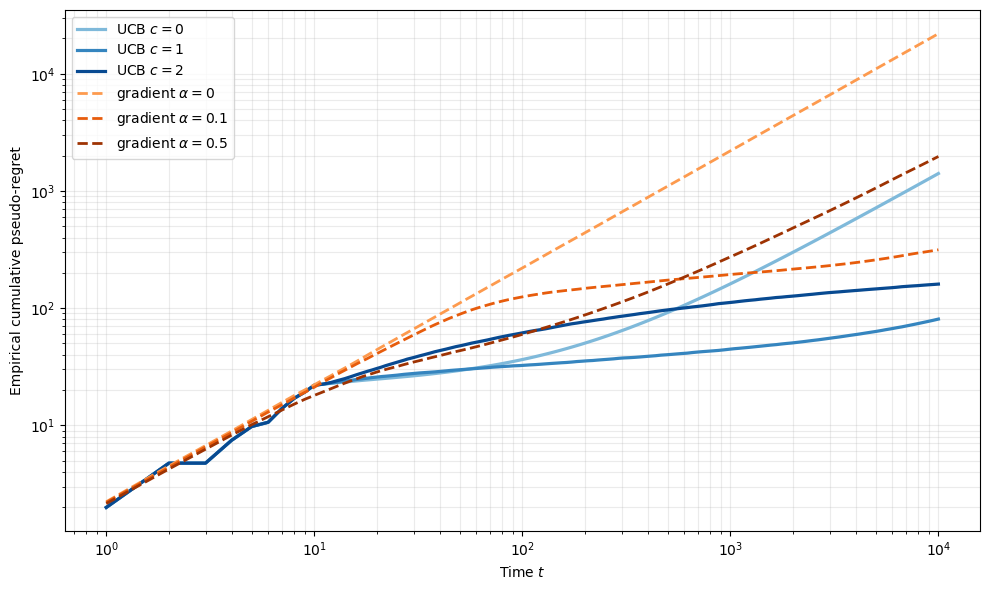
\includegraphics[width=0.76\linewidth]
    {figures/q6_gradient_vs_ucb_regret.png}
    \caption{Empirical cumulative pseudo-regret of the gradient-bandit
    and UCB algorithms over \(T=10^4\) time steps.}
    \label{fig:q6-gradient-ucb-regret}
\end{figure}

The cumulative pseudo-regret at \(T=10^4\) is summarised in
Table~\ref{tab:q6-regret}.

\begin{table}[H]
    \centering
    \caption{Empirical cumulative pseudo-regret at \(T=10^4\).}
    \label{tab:q6-regret}
    \begin{tabular}{lc}
        \toprule
        \textbf{Algorithm} & \textbf{Cumulative pseudo-regret} \\
        \midrule
        UCB, \(c=1\) & \(80.58\) \\
        UCB, \(c=2\) & \(160.29\) \\
        Gradient, \(\alpha=0.1\) & \(314.58\) \\
        UCB, \(c=0\) & \(1408.07\) \\
        Gradient, \(\alpha=0.5\) & \(1968.16\) \\
        Gradient, \(\alpha=0\) & \(21978.00\) \\
        \bottomrule
    \end{tabular}
\end{table}

Figure~\ref{fig:q6-gradient-ucb-regret} and
Table~\ref{tab:q6-regret} show that exploratory UCB achieves the lowest
regret: \(c=1\) gives \(80.58\), followed by \(c=2\) with \(160.29\).
The best gradient case, \(\alpha=0.1\), gives \(314.58\): about four times
the regret of UCB with \(c=1\), but well below non-exploratory UCB. The
larger \(\alpha=0.5\) result, \(1968.16\), shows greater sensitivity to
reward noise; with \(\alpha=0\), the policy stays uniform and regret is
approximately linear. Thus, for this instance and the tested parameters,
exploratory UCB gives the more regret-efficient trade-off.


\newpage

% ------------------------------------------------------------
% Question 7
% ------------------------------------------------------------

\section*{Question 7}
\questionequations{7}
% Online sync refresh: revised workshop report, 2026-08-29. figure-path-fix
To investigate the sensitivity of the gradient-bandit algorithm to the
learning rate, the experiment was repeated for
\[
    \alpha\in
    \{0.01,\,0.05,\,0.1,\,0.5,\,1,\,2,\,5\}.
\]
For each value of $\alpha$, the algorithm was run over $T=10^4$ time steps
and $M=300$ independent reruns. At each time step, the probability assigned
by the softmax policy to the true optimal arm
\[
    a^\ast\in\arg\max_{a\in\mathcal A}q^\ast(a)
\]
was recorded and averaged across reruns. Thus, convergence to the optimal
decision corresponds to the mean probability of selecting $a^\ast$
approaching one.

\begin{figure}[H]
    \centering
    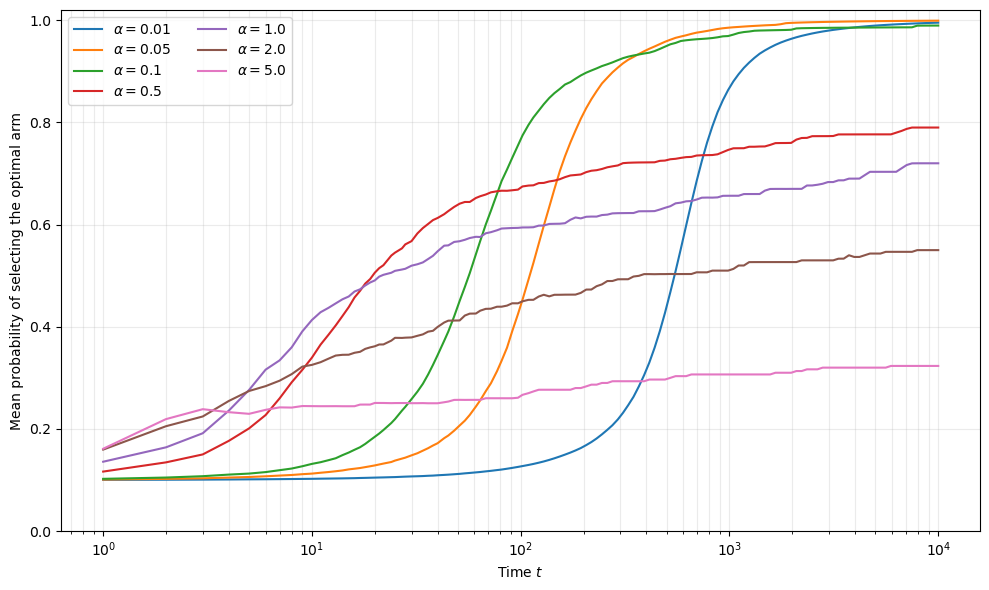
\includegraphics[width=0.92\linewidth]
    {figures/q7_gradient_alpha_sensitivity.png}
    \caption{Mean probability of selecting the optimal arm for different
    gradient-bandit learning rates.}
    \label{fig:q7-gradient-alpha}
\end{figure}

Figure~\ref{fig:q7-gradient-alpha} shows that satisfactory finite-horizon
concentration on the optimal arm is not obtained for every tested
$\alpha>0$. For the smaller learning rates
$\alpha=0.01$, $0.05$, and $0.1$, the probability of selecting the optimal
arm approaches approximately one by the end of the simulation. However,
performance deteriorates as the learning rate becomes large. At
$T=10^4$, the optimal-arm probabilities are only approximately $0.79$,
$0.72$, $0.55$, and $0.33$ for
$\alpha=0.5$, $1$, $2$, and $5$, respectively.

The mean curves hide a strongly bimodal run-level outcome. The final
probabilities are summarised in Table~\ref{tab:q7-concentration}.

\begin{table}[H]
    \centering
    \caption{Run-level concentration of the final optimal-arm probability
    $P_T(a^\ast)$ over $300$ reruns.}
    \label{tab:q7-concentration}
    \begin{tabular}{ccccc}
        \toprule
        $\alpha$ & Mean $P_T(a^\ast)$ & $P_T(a^\ast)>0.99$
        & $P_T(a^\ast)<0.01$ & Between \\
        \midrule
        $0.01$ & $0.9952$ & $1.0000$ & $0.0000$ & $0.0000$ \\
        $0.05$ & $0.9991$ & $1.0000$ & $0.0000$ & $0.0000$ \\
        $0.10$ & $0.9896$ & $0.9900$ & $0.0100$ & $0.0000$ \\
        $0.50$ & $0.7899$ & $0.7900$ & $0.2100$ & $0.0000$ \\
        $1.00$ & $0.7200$ & $0.7200$ & $0.2800$ & $0.0000$ \\
        $2.00$ & $0.5500$ & $0.5500$ & $0.4500$ & $0.0000$ \\
        $5.00$ & $0.3233$ & $0.3233$ & $0.6767$ & $0.0000$ \\
        \bottomrule
    \end{tabular}
\end{table}

For large $\alpha$, most reruns therefore assign either more than $0.99$ or
less than $0.01$ probability to the optimal arm, rather than fluctuating
around an intermediate policy. Large learning rates produce large
stochastic preference updates and often cause premature near-deterministic
concentration. Depending on early reward observations, this concentration
may be on either the optimal arm or a suboptimal arm.

Therefore, the numerical experiment demonstrates strong learning-rate
sensitivity for this bandit instance. Smaller tested values give behaviour
consistent with concentration on the optimal arm by $T=10^4$, whereas large
values frequently concentrate on a suboptimal arm. Since the experiment has
a finite horizon, it does not by itself prove a general asymptotic
convergence or non-convergence theorem for constant-step gradient bandits.


% ============================================================
% Appendix
% ============================================================

\newpage
\appendix
\input{appendix}

% ============================================================
% References
% ============================================================


\end{document}
